\chapter{Resultados}
\label{cap:Resultados}
En este capítulo se explican los resultados obtenidos en cada uno de los sprints del desarrollo del trabajo y cómo se relacionan con los objetivos definidos.

[... Hablar acerca de los sprints ...]


\section{Identificación y adquisición de las variables del sistema}
En el primer sprint se busca identificar cada una de las variables que entran en juego en el sistema, así como su proceso de obtención.. Se debe tener clara la diferencia entre variables de entrada y salida y variables de control.
\subsection{Variables de entrada}
Son las fuentes de suministro de energía al sistema. Habrá un total de tres:
\begin{itemize}
	\item \textbf{Energía fotovoltaica (EF)}\\ Energía procedente de las placas solares. Su valor viene determinado por varios factores, como son el número de módulos fotovoltaicos instalados y la máxima potencia posible en cada momento, \textit{current module power} (CMP). Hace referencia a la potencia de salida, en watios que produce un panel fotovoltaico en condiciones de máxima iluminación solar, con una radiación de aproximadamente 1 kW/m2. Será dependiente de la situación meteorológica del momento, de cuya obtención se hablará mas adelante. Como se puede observar, tendrá un valor máximo de obtención, que representa el tope de energía que podemos obtener de los módulos fotovoltaicos en ese momento.
	\item \textbf{Energía de red (ER)}\\ Energía procedente de la compañía eléctrica como cliente particular. Al contrario que en el caso anterior, no existe un límite superior a la hora de obtener energía de esta fuente.
	\item \textbf{Energía almacenada en batería (EB)}\\ Energía obtenida de la batería de almacenaje, que se ha guardado previamente para su posterior uso cuando el resto de fuentes de entrada tengan un mayor costo. Al igual que la energía fotovoltaica tiene un límite superior y viene determinado por la cantidad de carga de la misma y la profundidad de descarga que se le puede realizar sin resultar perjudicial para su ciclo de vida, que debe ser de un 50\% como máximo.
\end{itemize}

Cómo se ha mencionado, la energía fotovoltaica en una hora t será dependiente de la situación meteorológica de esa hora, algo evidente.\\Para obtener dicha información se utiliza la API oficial de AEMET \cite{Aemet}. Una API (\textit{Application Programming Interface}) es un conjunto de reglas o especificaciones que permite a las aplicaciones proporcionar servicios a otras o comunicarse. Para su uso, se ha debido solicitar un \textbf{API key} ya que es una API cerrada, esto es, su uso está restringido a un conjunto cerrado de clientes. Para realizar una petición a la misma, debe incluirse el \textit{API key} mencionado anteriormente en la url solicitada, así como una serie de parámetros como el código del municipio que se desea consultar. La respuesta a la petición contiene la previsión meteorológica de las próximas 24 horas en ese municipio.\\Para esta funcionalidad se ha creado el módulo \textit{api\_aemet}, que contiene la función \textit{get\_weather}, la cual se muestra en el listado~\ref{lst:aemet}
\begin{lstlisting}[language=Python,float=ht,caption={Función para obtener los valores meteorológicos},label={lst:aemet}]
def get_weather (city):
    weather_buffer = []
    url = const.AEMET_URL.replace('$CITY', city)
    response = requests.get(url)
    data = response.json()

    if data['estado'] == 200:
        url = data['datos']
        response = requests.get(url)
        data = response.json()[0]
        weather_buffer = create_weather_buffer(data)
        return weather_buffer
    return None
\end{lstlisting}
 Nótese que la url para la petición es obtenida como una constante de \textit{const}, alias que hace referencia al módulo de constantes del proyecto: \textit{project\_constants}. Este método realiza una petición a la API mediante la librería \textit{requests}~\cite{Kenn11}, y en caso de obtener un código de éxito (código de estado http 200), procesa la respuesta en la función \textbf{create\_weather\_buffer} y devuelve una lista con los 24 estados meteorológicos, correspondientes a las 24 horas de la simulación, del tipo: ["Despejado", "Poco Nuboso", "Despejado", ..., "Despejado"]\\

Las variables de entrada no son excluyentes, es decir, se puede obtener un tanto por ciento de la energía requerida procedente de cada una de ellas, lo que vendrá determinado por el precio en ese momento de cada una, ya que lo que buscamos es minimizar el gasto producido. A continuación se muestra el modo de determinación de los precios de las variables de entrada en una hora t: \\

	El precio de la energía fotovoltaica se calcula a partir de la inversión realizada en la instalación de los módulos fotovoltaicos y la cantidad de años en los que se desea amortizar dicha inversión. Así, el precio en €/Kw de EF se toma a partir de la fórmula~\ref{eq:costoEF}
	\begin{equation}
          \label{eq:costoEF}
	Costo_{EF} = \frac{coste_{anual}}{promedio^{kw}_{anual}} \textup{\euro}/kw
	\end{equation}
	Siendo el coste anual la cantidad invertida entre el número de años(n) en amortizarla, cómo se puede observar en la fórmula~\ref{eq:inversionEF}
	\begin{equation}
          \label{eq:inversionEF}
	Coste_{anual} = \frac{inversion}{n} \textup{\euro}
	\end{equation}


	El precio de la energía de red es el ya comentado PVPC. Para obtenerlo, se hace uso de la \textbf{API oficial de Red Eléctrica de España (e-sios)} \cite{Ree}. Para su uso se ha debido solicitar un \textit{Token} de acceso que se utiliza en las llamadas a la misma, al tratarse de una API cerrada análogamente al caso de la API de AEMET. Para el procesado de esta API se ha creado el módulo \textit{api\_esios}, que contiene la función \textit{get\_incoming\_prices}, la cuál se muestra en el listado~\ref{lst:esios}

	\begin{lstlisting}[language=Python,float=ht,caption={Función para obtener los valores del precio eléctrico},label={lst:esios}]
	def get_incoming_prices(indicator, start, end):
	   url = const.ESIOS_URL.replace('$INDICATOR', indicator)
	   url = url.replace('$START_DATE', dt.datetime.strftime(start, '%Y/%m/%d'))
	   url = url.replace('$END_DATE', dt.datetime.strftime(end, '%Y/%m/%d'))

	   response = requests.get(url, headers=HEADERS)
	   if response.status_code == 200:
	      data = response.json()
	      price_buffer = create_price_buffer(data, start)
	      return price_buffer
	   return None
	\end{lstlisting}

	Esta función es llamada desde el proyecto con el indicador deseado, que se corresponde con el precio que se desea consultar (en este caso PVPC), cuyo código numérico es obtenido de las constantes del proyecto, al igual que la url necesaria para la petición (ESIOS\_URL), que se forma con los parámetros adecuados y se realiza la petición \textit{get} haciendo uso de la librería \textit{requests}~\cite{Kenn11}. En este caso el \textit{API key} no se concatena en la url, si no que debe incluirse en la cabecera de la petición en un campo específico, ya que se trata de una autenticación por token como tal. Si la petición ha sido exitosa (código de respuesta http 200), la función retornará un \textit{buffer} de tamaño 24, que se corresponde con los valores del PVPC en las 24 horas definidas en la simulación. Para ello llama a \textit{create\_price\_buffer}, que se encargará de generar la lista con los 24 valores del precio solicitado procesando la respuesta recibida de la petición a la API.
	De esta manera se consigue el precio por Kw de la energía de red en cada momento.

	Por último, el precio de la energía de baterías se puede calcular de un modo muy parecido al de la energía fotovoltaica. Hace referencia al coste que supone extraer energía almacenada en la batería y está relacionado con la inversión realizada en la batería~\ref{eq:costoEB}
	\begin{equation}
          \label{eq:costoEB}
	Costo_{EB} = \frac{coste_{anual}}{capacidad_{bat}\cdot182,5} \textup{\euro}/kw
	\end{equation}
	Habiendo obtenido previamente el coste anual de forma similar a la fórmula~\ref{eq:inversionEF}. La constante 182,5 hace referencia al número de días del año (365) multiplicado por 0.5, debido a que no se va a realizar una profundidad de descarga mayor al 50\% de la capacidad total de la batería. El valor obtenido es el precio que supone recoger 1 Kw de la batería.
\subsection{Variables de salida}
Representan las fuentes de consumo de energía del sistema. Habrá un total de cuatro:
\begin{itemize}
\item \textbf{Consumo del hogar (C)}\\Demanda energética del hogar en cuestión, cuantía que debe ser satisfecha siempre, ya que es la energía que necesita el hogar para su uso cotidiano. En este trabajo fin de grado se ha decidido trabajar con clientes de la empresa eléctrica Endesa S.A., pues el hogar del alumno es su cliente lo que permitirá trabajar con información real. Además cuenta con un área privada de cliente que permite acceder a datos analíticos del hogar (Figura~\ref{fig:endesa}) y permite descargar ficheros en formato de texto con el consumo por horas de un día determinado en el hogar del cliente, justo lo que se necesita para dotar de valor esta variable. Para adaptar la información del fichero al valor de la variable se ha creado la función \textit{read\_from\_file(filename)} del módulo \textit{client\_consumption} que devuelve una lista con los 24 consumos de las 24 horas de la simulación en Kilowatios, obtenidos del fichero proporcionado.
  \begin{figure}[!h]
    \centering
    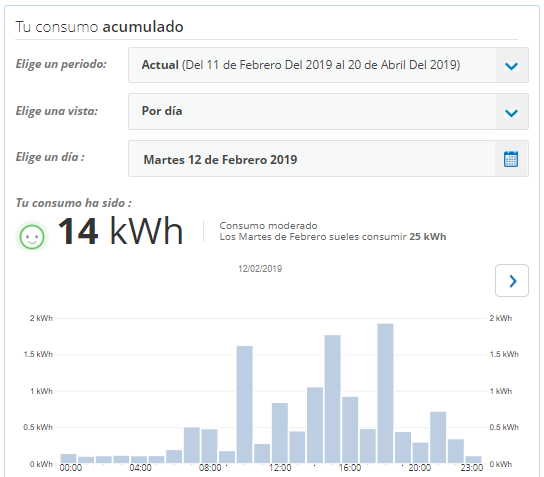
\includegraphics[width=10cm]{figs/Endesa.PNG}
    \caption{Panel de control del área cliente Endesa}
    \label{fig:endesa}
  \end{figure}
\item \textbf{Consumo interno del sistema ($ C_{int} $)}\\El sistema propuesto tiene un consumo constante de funcionamiento, cuyo valor se ha estimado en aproximadamente 2 Kw al día, alrededor de unos 0,088 watios por hora. Consta del consumo por funcionamiento de placas fotovoltaicas y realización de carga y descarga de batería.
	\item \textbf{Carga de batería (CB)}\\Cantidad de energía que se almacena en la batería para su posterior uso (almacenaje en batería). Esta variable cobra sentido en el caso de un abaratamiento de alguna fuente de generación de energía, lo que propicia que se obtenga más de la necesitada y se almacene para cuando el precio sea mayor.
	\item \textbf{Vertido al mercado eléctrico (CR)}\\Cantidad de energía que se vende al mercado eléctrico. Como particular, se puede disponer de una instalación fotovoltaica y verter energía a la red eléctrica, aunque es una práctica sujeta a numerosas trabas legales y dificultades en las que no se entrará en el desarrollo de este trabajo fin de grado. Esta energía se vertería al intramercado de red conocido como el mercado SPOT, aquel donde los activos que se compran o venden se entregan al precio de mercado del momento de la compra/venta.
\end{itemize}

Como se puede observar, el vertido al mercado eléctrico es un consumo que tiene un beneficio económico que ha de tenerse en cuenta. Existe una retribución por Kw vertido a la red dependiente del momento del día, ya que como se ha comentado antes, el valor de compra/venta del mercado SPOT varía. Para la obtención de estos valores se vuelve a hacer uso de la ya mencionada API e-sios, proporcionando a la función \textit{get\_incoming\_prices} el indicador del precio SPOT, presente en el fichero de constantes del proyecto. Análogo a la obtención del PVPC, se retorna un buffer con los 24 valores requeridos del precio SPOT correspondientes a las 24 horas a simular.\\

Aunque a priori parezca que el hecho de cargar las baterías no tiene una compensación económica, esto no es del todo correcto. Existe un beneficio económico, aunque no directo, con esta práctica. Puede ser explicado como la cantidad ahorrada por almacenar esa energía y no consumirla, ya que se ha pagado por ella. Este valor puede verse como el mínimo de los precios de las fuentes de generación de energía en el momento de la carga. Veamos un breve ejemplo:\\En la hora t se ha obtenido energía fotovoltaica a un precio de 0,11 € el Kwh. Por otro lado, se ha obtenido energía de la compañía eléctrica contratada a un precio de 0,14 € el Kwh. El beneficio económico indirecto por cargar un Kw de energía en batería en esta hora t será de 0,11 €.

\subsection{Variables de control}
Los valores de las variables definidas anteriormente son los que se intentan optimizar, pero existe otro conjunto de variables conocido como las variables de control. Aunque se denotan como variables, en el caso concreto de una simulación son constantes, ya que sus valores están predefinidos para la simulación del modelo. Este conjunto está formado por los valores de los que dependen las variables de entrada y salida y en función de los que se busca una optimización, y caracterizan tanto la simulación como la situación en una hora determinada.\\
Este conjunto está formado por:
\begin{itemize}
	\item \textbf{Fecha de inicio}\\ Valor que hace referencia al inicio de la simulación. Este valor es representado mediante el módulo datetime de Python. Datetime~\cite{Dtpy} es un módulo de la librería estándar de Python que permite manipular y trabajar con fechas. Este valor será un día y una hora de ese día.
	\item \textbf{Fecha de fin}\\ Corresponde al fin de la simulación. Siempre será 24 horas a partir de la fecha de inicio. Al igual que el anterior, se representa haciendo uso de datetime.
	\item \textbf{Número de módulos fotovoltaicos}\\ El número de módulos fotovoltaicos juega un papel fundamental. A mayor número de módulos, se producirá mas energía, pero mayor deberá ser la inversión para adquirirlos.
	\item \textbf{Precio de un módulo fotovoltaico}\\ En este trabajo el tipo de módulo fotovoltaico sera el se suele usar a nivel particular, de tamaño pequeño, con una potencia nominal en condiciones ideales de 50 watios hora~\ref{fig:pv_module}. Este modulo tiene un precio por unidad de 40 €, por lo tanto este valor tendrá el mismo valor en todas las simulaciones.
          \begin{figure}[!h]
            \centering
            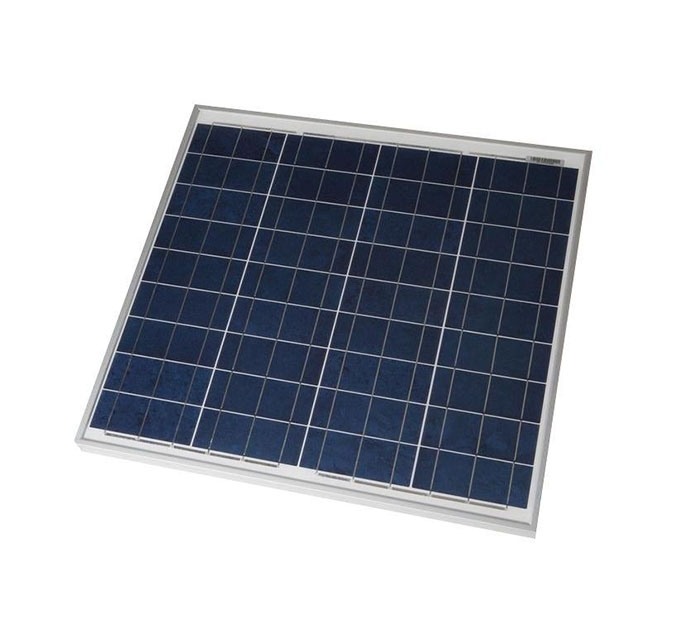
\includegraphics[width=6cm]{figs/panel_solar.jpg}
            \caption{Panel fotovoltaico de 50 W}
            \label{fig:pv_module}
          \end{figure}
	\item \textbf{Años en amortizar la inversión de los módulos fotovoltaicos}\\ El número de años en los que se desea amortizar la inversión realizada en la adquisición de los módulos fotovoltaicos, exclusivamente mediante su uso. Como se ha comentado anteriormente, no es algo trivial ya que determinará en gran medida el precio de extracción de energía fotovoltaica.
	\item \textbf{Precio de la batería}\\ En este trabajo el tipo de batería usado será una batería estacionaria~\ref{fig:bateria} compuesta por plomo abierto y gel. Este tipo de batería esta compuesta por dos vasos de 2V cada uno que disponen de un amplio rango de autonomía y una vida útil bastante larga, alrededor de unos 20 años. Son aconsejadas en instalaciones con un consumo medio (microondas, horno, lavadora, aire acondicionado, etc), es decir, perfectas para un hogar de tamaño normal. Cómo su tensión es de 2V, se debe instalar un total de 6 vasos en serie, al estar la instalación solar a 12V. Su precio es elevado debido a la gran capacidad, siendo un precio de 7900 € el de la obtención de los 6 vasos.
           \begin{figure}[!h]
            \centering
            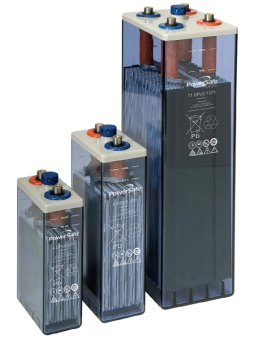
\includegraphics[width=4cm]{figs/bateria.jpg}
            \caption{Batería estacionaria}
            \label{fig:bateria}
          \end{figure}
	\item \textbf{Capacidad de la batería}\\ El tipo de batería usado, es decir, batería estacionaria de 6 vasos, tiene una capacidad total de aproximadamente 21 Kw. La profundidad de descarga de este tipo de batería es aproximadamente del 50\%, esto es, como se comento durante la explicación de las variables de entrada y salida, el tanto por ciento que se puede descargar dicha batería sin resultar perjudicial para su salud y por lo tanto afectar a su ciclo de vida útil.
	\item \textbf{Nivel de carga inicial de la batería}\\ Variable de control que define el estado inicial de la batería a la hora de realizar la simulación del modelo. Esto es la cantidad de energía que tiene almacenada la misma.
	\item \textbf{Años en amortizar la inversión de la batería}\\ Como ocurre en el caso de la inversión fotovoltaica, se debe determinar el número de años en los que se desea realizar la amortización de la inversión por adquirir la batería. Al tratarse de un valor mucho mas elevado debe ser mayor al del caso anterior, ya que si no se dispararía el precio de descargar las baterías y dejaría de ser una entrada a tener en cuenta al no resultar rentable.
\end{itemize}
Con esto quedan identificadas cada una de las variables que entran en juego en el modelo, así como su medio de adquisición.

\section{Aplicación de lógica difusa para la determinación de los estados meteorológicos}
En el segundo sprint se describe el procedimiento llevado a cabo para el uso de los estados meteorológicos obtenidos de la API de AEMET~\cite{Aemet}.

Tal y como se comentó en el sprint anterior, la respuesta a la petición \textit{requests} recibida por dicha API consta de estados meteorológicos en formato de cadena de texto. Un ejemplo de respuesta se muestra (simplificado) en el listado 4.3. (\textcopyright AEMET)

\begin{lstlisting}[numbers=none,caption={Ejemplo de respuesta de la API - AEMET}]]
{
 origen: {
	productor: "Agencia Estatal de Meteorología - AEMET. Gobierno de España",
	web: "http://www.aemet.es",
	language: "es",
	copyright: "AEMET. Autorizado el uso de la información y su reproducción citando a AEMET como autora de la misma.",
	notaLegal: "http://www.aemet.es/es/nota_legal"
 },
 elaborado: "2019-2-12",
 nombre: "Consuegra",
 provincia: "Toledo",
 prediccion: {
 	dia: [
		{
		 estadoCielo: [
					{
					 periodo: "08",
					 descripcion: "Cubierto"
					},
					{
					 periodo: "09",
					 descripcion: "Cubierto con lluvia escasa"
					},
					{
					 periodo: "10",
					 descripcion: "Cubierto con lluvia escasa"
					},
					{
					 periodo: "11",
					 descripcion: "Cubierto"
					},
					...
		 ]
		}
	}
}
\end{lstlisting}

Cómo se puede observar, en el campo 'predicción' existe un subcampo 'estadoCielo' (entre otros que se han obviado por no ser de interés en este trabajo) que contiene una lista con los estados meteorológicos. Cada elemento de la lista contiene dos valores: período (hora del día de esa previsión) y descripción (cadena de texto que describe el estado del cielo). Claramente existe un problema, ya que para la determinación de la máxima energía fotovoltaica posible en una hora determinada debe conocerse la potencia nominal posible (potencia que es capaz de suministrar el módulo fotovoltaico), directamente proporcional al estado meteorológico, el cuál es un texto que describe la situación y no un valor numérico que representa los watios que puede dar un módulo en esas condiciones, y a priori no se dispone de una forma directa de relacionarlas. \\

Se emplea \textbf{lógica difusa} para poder resolver la problemática mencionada anteriormente.
\subsection{Lógica difusa}
La teoría de la lógica difusa proporciona un marco matemático que permite modelar la incertidumbre de los procesos cognitivos humanos para poder ser tratable por un computador. Estos procesos cognitivos hacen referencia a expresiones del tipo:
\begin{itemize}
	\item Si no vives \textit{lejos} puedes ir en bicicleta. 
	\item Si hace \textit{mucho} frío llévate un chaquetón. 
\end{itemize} 
Los humanos son capaces de interpretar estos valores rápidamente, aunque no existe un valor cuantitativo que indique la distancia a la que se refiere la palabra \textit{lejos} o cuánto es \textit{mucho} frío. Sin embargo, las máquinas tienen algún que otro problema. Si se intentan trasladar estas reglar a código, aparecen dificultades ya que no se puede procesar numéricamente. Una opción es definir intervalos de valores que comprende cada palabra (por ejemplo, tomando \textit{lejos} como la distancia comprendida entre 5 y 10 kilómetros), pero esto no es preciso ya que para un computador, la distancia de 5,01 kilómetros sería lejos rotundamente, cuando en realidad la interpretación correcta no es así. Con ésto queda a la vista que la lógica convencional no trata de forma eficiente este problema. La solución pasa por emplear un método de razonamiento afín a la lógica difusa. \\

La lógica difusa permite representar matemáticamente la \textbf{incertidumbre}, mediante el empleo de herramientas formales. Según Zadeh~\cite{Zad73}, "\textit{Cuando aumenta la complejidad, los enunciados precisos pierden su significado y los enunciados útiles pierden precisión.}", es decir, \textit{los árboles no te dejan ver el bosque}, pues prácticamente cualquier problema del mundo puede resolverse partiendo de unas variables de entrada y buscando obtener como objetivo un conjunto de variables de salida. La lógica difusa establece esa relación entre variables de forma correcta.

\subsection{\textit{Fuzzy Sets}}



\begin{figure}[!h]
	\centering
	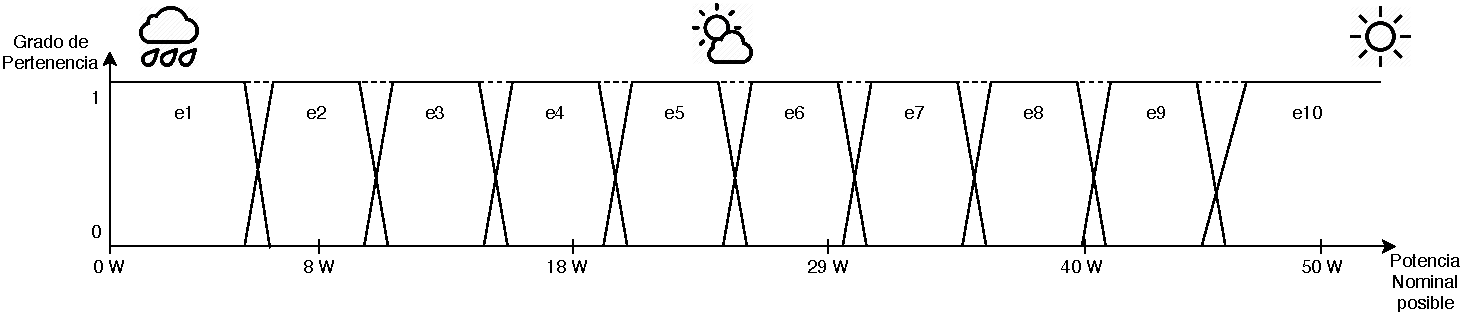
\includegraphics[width=17cm]{figs/Fuzzy_diagram.pdf}
	\caption{\textit{Fuzzy sets de los estados meteorológicos}}
\end{figure}
\section{Creación de las relaciones y restricciones propias del modelo}
Cómo se comento en el capítulo relativo al Objetivo del trabajo fin de grado, éste se aborda como un \textbf{problema de satisfacción de restricciones}.\\

La programación por restricciones es una metodología software que permite resolver problemas de gran complejidad, típicamente NP. Ésta metodología ha generado mucha espectación en el área de la inteligencia artificial desde la década de los 60, ya que tiene un gran potencial para la resolución de problemas reales. La idea básica de la programación por restricciones es primero declarar una serie de restricciones sobre el dominio del problema que atañe, para después dar con soluciones que satisfacen las anteriores restricciones de la forma más optima posible. Así, un problema de satisfacción de restricciones~\cite{Russ06} está caracterizado por:
\begin{itemize}
	\item Un conjunto de variables, donde cada variable dispone de un dominio de valores que puede tomar.
	\item Un conjunto de restricciones, que permite conocer las posibles combinaciones de las variables.
	\item La solución al PSR será la asignación de valores a las variables de forma que se satisfacen las restricciones y se alcanza el objetivo, representado típicamente como una función a optimizar.
\end{itemize}
Las restricciones se caracterizan por su \textbf{aridad}, que viene a ser el número de variables que involucra. Pudiendo ser unarias, si solo involucran una variable; binarias, si involucran dos variables; y n-arias, si involucran más de dos variables. Se deben tener en cuenta un tipo de restricción adicional, ya que están presentes en este trabajo, como son las \textbf{restricciones lineales}, expresadas teóricamente de la forma~\ref{eq:rest_lineal}
\begin{equation}
  \label{eq:rest_lineal}
  \sum_{i}^{n} a_{i}x_{i} (<,\leq,=,\geq,>,\neq) c
\end{equation}
siendo a el coeficiente de la variable x y c constante.\\

\subsection{Variables del PSR}

En los sprints 1 y 2 se identificaron las variables del problema, las cuáles están divididas en tres grupos: variables de entrada, variables de salida y variables de control. Sin embargo conviene mencionar cuáles de estas variables son las propias del problema de satisfacción de restricciones, y cuáles formarán las restricciones. El objetivo del problema es obtener valores de energía para los paneles fotovoltaicos, baterías y red eléctrica, de tal modo que se cubra la demanda energética del hogar y que el gasto económico sea el menor. Es por esto que las variables propias del problema de satisfacción de restricciones serán:
\begin{itemize}
\item \textbf{Energía fotovoltaica (EF)}. Energía obtenida de los módulos fotovoltaicos.~\ref{eq:dom_ef}
\begin{equation}
        \label{eq:dom_ef}
        Dom_{EF} = [0, EF_{max}]
\end{equation}
\item \textbf{Energía de red (ER)}. Energía importada de la red eléctrica.~\ref{eq:dom_er}
\begin{equation}
        \label{eq:dom_er}
        Dom_{ER} = [0, +\infty)
\end{equation}
\item \textbf{Energía de batería (EB)}. Energía obtenida de la batería.~\ref{eq:dom_eb}
\begin{equation}
        \label{eq:dom_eb}
        Dom_{EB} = [0, +\infty)
\end{equation}
\item \textbf{Consumo de batería (CB)}. Energía consumida para cargar la batería.~\ref{eq:dom_cb}
\begin{equation}
        \label{eq:dom_cb}
        Dom_{CB} = [0, +\infty)
\end{equation}
\item \textbf{Consumo de red (CR)}. Energía vertida a red a cambio de retribución económica.~\ref{eq:dom_cr}
\begin{equation}
        \label{eq:dom_cr}
        Dom_{CR} = [0, +\infty)
\end{equation}
\end{itemize}

Las restricciones estarán definidas en función de dichas variables y cada solución al problema estará formada por un valor para cada una de estas variables. Éstos valores satisfacen las restricciones y además serán los óptimos para que se produzca el menor gasto económico posible. El resto de variables (variables de control) determinarán las propias restricciones y el valor de las anteriores dependerá de éstas en una hora concreta t, entre 0 y 24h.\\

\subsection{Restricciones del PSR}
A continuación se determinan las restricciones a las que está sometido el modelo en una hora t:
\begin{itemize}
\item \textbf{Toda la energía generada debe ser consumida}.~\ref{eq:restr1}\\ \\Hace referencia al principio básico de la energía, la energía que se produce se consume de un modo u otro, no es posible que la suma de las variables correspondientes a la generación de energía (EB, ER y EF) sea distinta a la suma de las variables que hacen referencia al consumo de energía (CR, CB, $ C_{int} $ y C). Ésto debe producirse en cada una de las horas de la simulación. Así, tenemos una restricción lineal y n-aria correspondiente a la suma de las 24 horas correspondientes a una simulación, por lo que ésta restricciones a efectos prácticos es tomada como 24 restricciones a cumplir.
\begin{equation}
        \label{eq:restr1}
        \sum_{i=0}^{23} EF_{i}+ER_{i}+EB_{i} = CR_{i}+CB_{i}+C_{int}+C
\end{equation}

\item \textbf{No se puede producir energía fotovoltaica durante la noche}.~\ref{eq:restr2}\\ \\Algo obvio, pues sin luz solar la energía fotovoltaica no es posible. Ésto no está controlado en la API AEMET, ya que las peticiones relativas a la noche no reflejan una descripción propia del tiempo nocturo, si no que devuelve los mismos valores independientemente de si existe luz solar, por lo que debe manejarse mediante una restricción. Para este trabajo las horas de la noche serán las pertenecientes al intervalo temporal desde las 22:00 pm hasta las 7:00 am. Cómo posible trabajo futuro, podría determinarse este intervalo en función de la estación del año para que pueda ser un intervalo con mayor grado de efectividad. Se trata de una restricción unaria, donde para ciertos valores de t, EF debe ser 0. Es por esto que esta restricción a efectos prácticos es tomada como 9 restricciones (las 9 horas de noche definidas anteriormente)
\begin{equation}
        \label{eq:restr2}
        EF_{noche} = 0
\end{equation}

\item \textbf{La energía fotovoltaica generada no puede ser mayor que la máxima energía fotovoltaica en t}.~\ref{eq:restr3}\\ \\No se puede superar el umbral de generación de energía fotovoltaica establecido por la potencia nominal máxima de esa hora t, pues se estaría violando la capacidad real de producción de los módulos fotovoltaicos del sistema. Es una restricción lineal unaria, ya que la energía fotovoltaica máxima de cada hora t es constante, pues como se comentó anteriormente, sólo es dependiente del número de módulos fotovoltaicos y la situación meteorológica (obtenida de la API AEMET). A efectos prácticos, esta restricción es tomada como 24 restricciones a cumplir referentes a las 24 horas de la simulación.
\begin{equation}
        \label{eq:restr3}
        \sum_{i=0}^{23} EF_{i} \leq EF_{i}^{max}
\end{equation}

\item \textbf{La energía obtenida de la batería no puede ser mayor que el nivel de batería actual teniendo en cuenta la profundidad máxima de descarga}.~\ref{eq:restr4}\\ \\Básicamente no se puede obtener una cantidad de energía mayor a la posible en esa hora t, que vendrá determinada por la diferencia entre el  nivel de carga disponible al comienzo de esa hora y la capacidad máxima de la batería por la profundidad de descarga (50\%), para evitar daños en su ciclo de vida útil. Restricción unaria, pues solo involucra la variable EB, ya que el resto de elementos de la restricción son constantes en una hora t (nivel de carga actual, capacidad máxima de la batería y profundida de descarga). Al igual que las restricciones anteriores es lineal y a efectos prácticos representa 24 restricciones a cumplir.
\begin{equation}
        \label{eq:restr4}
        \sum_{i=0}^{23} EB_{i} \leq nivel_{i-1} - capacidad_{max} * profundidad_{descarga}
\end{equation}

\item \textbf{El consumo para cargar la batería no puede ser mayor que la capacidad de la misma menos el nivel restante después de t}.~\ref{eq:restr5}\\Parecido a la restricción anterior, en esta se modela el hecho de cargar la batería (CB) en cada hora t, el cuál está condicionado por la cantidad de batería restante para completar la carga (100\%), obtenido mediante la diferencia entre la capacidad máxima de la misma y lo consumido en la hora t (nivel de carga antes de comenzar la hora t menos la energía consumida de batería en t). Restricción binaria pues involucra tanto el consumo de batería (CB) como la energía de batería (EB), siendo la capacidad máxima de la batería y el nivel de carga en t constantes. Es tomado como 24 restricciones ya que debe cumplirse en cada una de las 24 horas de una simulación.
\begin{equation}
        \label{eq:restr5}
        \sum_{i=0}^{23} CB_{i} \leq capacidad_{max}- (nivel_{i-1} - EB_{i})
\end{equation}

\end{itemize}

Por lo tanto, a efectos prácticos, el PSR tiene 81 restricciones que satisfacer para determinar los valores de las variables.

\subsection{Función Objetivo}
Cómo se ha comentado antes, un problema de satisfacción de restricciones está determinado por un conjunto de variables y sus dominios, un conjuntos de restricciones de esas variables, y un objetivo. Por el momento se dispone de los dos primeros, por que en este apartado se procede a determinar el último, \textbf{la función objetivo}.\\

Un PSR que cuenta únicamente con variables y restricciones para esas variables podrá tener numerosas soluciones, representadas como una tupla con valores para cada variable. Añadiendo un objetivo al PSR se consigue unificar la solución, pues de todas esas soluciones, sólo una optimizará un objetivo concreto, y contendrá los valores óptimos de cada variable para ello.\\

Como se ha comentado a lo largo del desarrollo de este trabajo fin de grado, el objetivo del problema es \textbf{minimizar el gasto económico} producido mediante la optimización de energía en cada simulación de 24 horas, por lo tanto se buscarán valores de las variables que, además de satisfacer el conjunto de restricciones, sean óptimos para que el gasto económico sea mínimo. Éste gasto económico es dependiente del precio en la hora t de cada una de las energías que representan las variables. De estos precios se habló y se implementó la forma de obtenerlos en el sprint 1. Sus valores son constantes en cada hora t. Dicho esto, la función objetivo a minimizar está formada por el sumatorio de los gastos económico en cada hora t, por lo que representa el gasto económico de toda la simulación.~\ref{eq:funcionObjetivo}
\begin{equation}
\label{eq:funcionObjetivo}
f(x) = \sum_{i=0}^{23} EF_{i}P_{i}^{F} + ER_{i}P_{i}^{R_{PVPC}} + EB_{i}P_{i}^{B_{out}} - CB_{i}P_{i}^{B_{in}} - CR_{i}P_{i}^{R_{SPOT}}
\end{equation}
Siendo:
\begin{itemize}
\item $ EF_{i}P_{i}^{F} $: Gasto económico producido al generar energía fotovoltaica en la hora t.
\item $ ER_{i}P_{i}^{R_{PVPC}} $: Gasto económico producido al importar energía a la compañía eléctrica en la hora t.
\item $ EB_{i}P_{i}^{B_{out}} $: Gasto económico producido al descargar la batería en la hora t.
\item $ CB_{i}P_{i}^{B_{in}} $: Ganancia económica producida al cargar la batería en la hora t.
\item $ CR_{i}P_{i}^{R_{SPOT}} $: Ganancia económica producida al verter energía al mercado eléctrico en la hora t.
\end{itemize}

En cada simulación se buscará que el valor de $ f(x) $ sea el menor posible y la solución al PSR de esa simulación será los valores que deben tomar las variables para hacerlo posible.

\subsection{Implementación de la clase Simulation}
Vistos los apartados anteriores, es la hora de implementar una clase para representar el modelo de simulación, y poder crear objetos que representan una simulación concreta. Esta clase se llama \textbf{Simulation}~\ref{fig:simulation} y está disponible en el módulo simulation.\\

Los atributos de clase de Simulation serán las variables de control que tendrá cada objeto correspondiente a una simulación:
\begin{itemize}
        \item start: variable de control referente a fecha de inicio de la simulación. Es de tipo datetime.
        \item end: variable de control referente a fecha de fin de la simulación. Al igual que start, es una variable de formato fecha (datetime).
        \item ef\_price: variable de control referente al precio de generar energía fotovoltaica. Se trata de un número tipo float, pues tendrá el mismo valor en toda la simulación (se obtiene a partir de la inversión realizada)
        \item er\_price: variable de control referente a los precios que tendrá el PVPC en cada hora de la simulación. Es una lista de 24 elementos de tipo float.
        \item eb\_price: variable de control referente al precio de descargar la batería. Es un número de tipo float ya que será igual en las 24 horas de la simulación.
        \item cr\_price: variable de control referente a los precios SPOT en cada hora de la simulación, es decir, el precio del vertido de energía a la red eléctrica.
        \item cb\_price: variable de control referente a los precios de cargar la batería. Cómo es dependiente de los precios de energía fotovoltaica y de red de cada hora t, se trata de una lista con 24 valores.
        \item battery\_capacity: variable de control referente a la capacidad total de la batería. Variable de tipo float.
        \item battery\_level: variable de control que representa el nivel inicial de carga de la batería. Variable de tipo float.
        \item discharge\_depth: variable de control referente a la profundidad de descarga permitida en la batería. Variable de tipo float.
        \item max\_ef\_buffer: Más que una variable de control, representa los 24 valores máximos posible de energía fotovoltaica, obtenidos como se comentó anteriormente mediante la información de la API AEMET y el número de módulos fotovoltaicos, por ende, se trata de una lista de 24 valores.
        \item c\_int: referente a la variable de control del consumo interno del sistema. Variable de tipo float.
        \item c: referente al consumo del hogar, lista de los 24 valores con el consumo del hogar en las 24 horas de la simulación.

Las funciones de esta clase sirven para calcular algunos de los atributos anteriores. En la figura~\ref{fig:simulation} se muestra la clase UML de Simulation.
\end{itemize}

\begin{figure}[H]
        \centering
        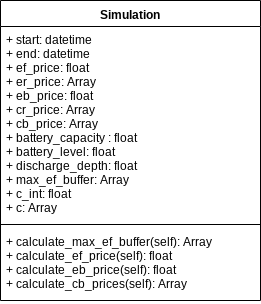
\includegraphics[width=6cm]{figs/simulation_class.png}
        \caption{Clase Simulation}
        \label{fig:simulation}
\end{figure}

En el próximo sprint se implementará cada una de las restricciones para permitir ejecutar la simulación.

\section{Generación optimizada de energía mediante programación lineal}
Cómo se comentó anteriormente, éste PSR dispone de 81 restricciones. Además, no interesa cualquiera de las soluciones posibles si no que debe buscarse la solución más óptima de todas. Por lo tanto para su resolución deberá emplearme algún procedimiento lo suficientemente potente para contemplar ambos requisitos.
\subsection{Programación Lineal}
La programación lineal~\cite{Loom64} tiene como objetivo optimizar una función lineal cuyas variables están sujetas a un conjunto de restricciones lineales.
Se trata de un campo de la matemática muy efectivo para la resolución de problemas donde se desea sacar el mayor provecho de una situación.\\

Historicamente, el concepto de programación lineal debe su nombre a John Von Neumann (1947), uno de los matemáticos más importantes del siglo XX gracias a sus contribuciones en las ciencias de la computación; y a George Dantzig (1947), cuyo trabajo intentaba asignar 70 puestos de trabajo a 70 personas mediante programación lineal. Las permutaciones necesarias para la asignación óptima de dichos puestos era factorial de 70 (70!), algo enorme, pues el número de combinaciones de variables es inmenso. Curiosamente, mediante programación lineal el problema se resuelve en un momento pues el número de combinaciones se reduce en su mayor parte. La programación lineal puede ser aplicable a numerosos problemas comunes tales como:
\begin{itemize}
\item Asignación de horarios a profesores en un centro educativo para obtener la mayor productividad a la par que comodidad para profesor y alumno.
\item Distribución de elementos en almacenes de tal modo que se reduzca el costo de almacenamiento teniendo en cuenta la limitada capacidad.
\item Distribución de bienes entre compradores y consumidores de tal modo que las ganancias del intermediario sean máximas.
\end{itemize}
Cómo se puede observar, el problema de este trabajo fin de grado está muy relacionado con el último ejemplo, pues se distribuye cantidad de energía entre fuentes de entrada y fuentes de salida de manera óptima para garantizar un gasto mínimo de consumo energético.\\

Para un problema de programación lineal pueden existir varios casos en su resolución:
\begin{itemize}
\item Existe una solución óptima.
\item Existen varias soluciones óptimas.
\item No existe solución.
\item Existen soluciones infitas.
\end{itemize}
La situación deseada es la primera, pero puede ocurrir alguno de los otro casos. Estas situaciones pueden resolverse convirtiendo las restricciones que son inecuaciones (desigualdades) en igualdades.\\

Existen varios métodos de programación lineal. El más utilizado es conocido como el \textbf{método Simplex}, pues es muy potente debido a que se basa en evaluar solo algunos puntos extremos mediante dos condiciones:
\begin{itemize}
\item \textbf{Optimalidad}. La solución inferior relativa al punto de solución actual no se tiene en cuenta.
  \item \textbf{Factibilidad}. Una vez se encuentra una solución básica factible, sólo apareceran soluciones factibles.
\end{itemize}
Otro método de programación lineal es el método de ramificación y acotamiento \textit{branch and bound}, el cuál divide el problema en varios subproblemas de programación lineal, acotamiento que permite obtener soluciones óptimas que se mejorar por cada subproblema.\\

En el ámbito de las ciencias de la computación existen librerías que permiten emplear algoritmos de programación lineal para la resolución de problemas de optimización. En este trabajo fin de grado se empleará la librería del lenguaje Python \textbf{Scipy}.

\section{Persistencia de datos y creación del servidor}
Una vez implementada la funcionalidad de simulación, debe pensarse en añadir una persistencia al proyecto de los elementos que intervienen. Esto es necesario y primordial si se pretende crear una aplicación web para realizar simulaciones. Puesto que se creará una API usando Flask~\cite{Flask} que hará la función de servidor, se ha dedicido utilizar la herramienta para gestión de base de datos SQLAlchemy.
\subsection{Persistencia con SLQAlchemy}
SQLAlchemy~\cite{SqlAl} proporciona un kit de herramientas SQL que permiten manejar bases de datos de manera eficiente. Está formado por dos componentes:
\begin{itemize}
\item \textit{Core}: Es un conjunto de herramientas de SQL que da lugar a un nivel de abstracción sobre el mismo, mediante un lenguaje que utiliza expresiones generativas en Python para expresar órdenes SQL.
\item \textit{ORM}: Se trata de un asignador relacional de objetos, es decir, permite crear una base de datos de objetos virtuales que permite manipular la información de la base de datos, a priori incompatible, como objetos utilizable por un lenguaje de programación orientada a objetos.
\end{itemize}
Mediante las consultas basadas en funciones permite ejecutar las cláusulas SQL mediante funciones y expresiones en Python. Se pueden realizar numerosas acciones como subconsultas seleccionables, insertar, actualizar, eliminar o declarar un objeto, combinaciones internas y externas. El ORM permite almacenar en caché las colecciones y referencias de objetos una vez han sido cargados, dando lugar a que no sea necesario emitir SQL en cada acceso.\\

SQLAlchemy puede trabajar con bases de datos de SQLite, Postgresql, MySQL, Oracle, MS-SQL, Sybase y Firebird, entre otros.
\subsection{Modelos User y Home}
\subsection{Creación de API con Flask}
\subsection{Desarrollo de la interfaz web}

\section{Migración de la aplicación a un contenedor Docker integrado en la nube}
